\documentclass[12pt]{article} 
% \documentclass[12pt]{amsart} 

% Custom definitions
% To use this customization file, insert the line "% Custom definitions
% To use this customization file, insert the line "% Custom definitions
% To use this customization file, insert the line "\input{custom}" in the header of the tex file.

% Formatting

\tolerance=1000
\usepackage[margin=1in]{geometry}


% Packages

% \usepackage{amssymb,latexsym}
\usepackage{amssymb,amsfonts,amsmath,latexsym,amsthm}
\usepackage[usenames,dvipsnames]{color}
\usepackage[]{graphicx}
\usepackage[space]{grffile}
\usepackage{mathrsfs}   % fancy math font
% \usepackage[font=small,skip=0pt]{caption}
\usepackage[skip=0pt]{caption}
\usepackage{subcaption}
\usepackage{verbatim}
\usepackage{url}
\usepackage{bm}
\usepackage{dsfont}
\usepackage{extarrows}
\usepackage{multirow}
% \usepackage{wrapfig}
% \usepackage{epstopdf}
\usepackage{rotating}
\usepackage{tikz}
\usetikzlibrary{fit}					% fitting shapes to coordinates
%\usetikzlibrary{backgrounds}	% drawing the background after the foreground

\usepackage{fancyhdr}

\fancypagestyle{firststyle}{
   \fancyhf{}
   \renewcommand{\footrulewidth}{0.4pt}
   \fancyfoot[L]{\footnotesize This work is licensed under a \href{http://creativecommons.org/licenses/by-nc-nd/4.0/}{Creative Commons BY-NC-ND 4.0 International License}.\\ Jeffrey W. Miller (2015). \textit{Lecture Notes on Bayesian Statistics}. Duke University, Durham, NC.}
}


% \usepackage[dvipdfm,colorlinks,citecolor=blue,linkcolor=blue,urlcolor=blue]{hyperref}
\usepackage[colorlinks,citecolor=blue,linkcolor=blue,urlcolor=blue]{hyperref}
%\usepackage{hyperref}
\usepackage[authoryear,round]{natbib}


%  Theorems, etc.

\theoremstyle{plain}
\newtheorem{theorem}{Theorem}[section]
\newtheorem{corollary}[theorem]{Corollary}
\newtheorem{lemma}[theorem]{Lemma}
\newtheorem{proposition}[theorem]{Proposition}
\newtheorem{condition}[theorem]{Condition}
% \newtheorem{conditions}[theorem]{Conditions}

\theoremstyle{definition}
\newtheorem{definition}[theorem]{Definition}
% \newtheorem*{unnumbered-definition}{Definition}
\newtheorem{example}[theorem]{Example}
\theoremstyle{remark}
\newtheorem*{remark}{Remark}
\numberwithin{equation}{section}



% Document-specific shortcuts
\newcommand{\btheta}{{\bm\theta}}
\newcommand{\bbtheta}{{\pmb{\bm\theta}}}

\newcommand{\commentary}[1]{\ifx\showcommentary\undefined\else \emph{#1}\fi}

\newcommand{\term}[1]{\textit{\textbf{#1}}}

% Math shortcuts

% Probability distributions
\DeclareMathOperator*{\Exp}{Exp}
\DeclareMathOperator*{\TExp}{TExp}
\DeclareMathOperator*{\Bernoulli}{Bernoulli}
\DeclareMathOperator*{\Beta}{Beta}
\DeclareMathOperator*{\Ga}{Gamma}
\DeclareMathOperator*{\TGamma}{TGamma}
\DeclareMathOperator*{\Poisson}{Poisson}
\DeclareMathOperator*{\Binomial}{Binomial}
\DeclareMathOperator*{\NormalGamma}{NormalGamma}
\DeclareMathOperator*{\InvGamma}{InvGamma}
\DeclareMathOperator*{\Cauchy}{Cauchy}
\DeclareMathOperator*{\Uniform}{Uniform}
\DeclareMathOperator*{\Gumbel}{Gumbel}
\DeclareMathOperator*{\Pareto}{Pareto}
\DeclareMathOperator*{\Mono}{Mono}
\DeclareMathOperator*{\Geometric}{Geometric}
\DeclareMathOperator*{\Wishart}{Wishart}

% Math operators
\DeclareMathOperator*{\argmin}{arg\,min}
\DeclareMathOperator*{\argmax}{arg\,max}
\DeclareMathOperator*{\Cov}{Cov}
\DeclareMathOperator*{\diag}{diag}
\DeclareMathOperator*{\median}{median}
\DeclareMathOperator*{\Vol}{Vol}

% Math characters
\newcommand{\R}{\mathbb{R}}
\newcommand{\Z}{\mathbb{Z}}
\newcommand{\E}{\mathbb{E}}
\renewcommand{\Pr}{\mathbb{P}}
\newcommand{\I}{\mathds{1}}
\newcommand{\V}{\mathbb{V}}

\newcommand{\A}{\mathcal{A}}
\newcommand{\C}{\mathcal{C}}
\newcommand{\D}{\mathcal{D}}
\newcommand{\Hcal}{\mathcal{H}}
\newcommand{\M}{\mathcal{M}}
\newcommand{\N}{\mathcal{N}}
\newcommand{\X}{\mathcal{X}}
\newcommand{\Zcal}{\mathcal{Z}}
\renewcommand{\P}{\mathcal{P}}

\newcommand{\T}{\mathtt{T}}
\renewcommand{\emptyset}{\varnothing}


% Miscellaneous commands
\newcommand{\iid}{\stackrel{\mathrm{iid}}{\sim}}
\newcommand{\matrixsmall}[1]{\bigl(\begin{smallmatrix}#1\end{smallmatrix} \bigr)}

\newcommand{\items}[1]{\begin{itemize} #1 \end{itemize}}

\newcommand{\todo}[1]{\emph{\textcolor{red}{(#1)}}}

\newcommand{\branch}[4]{
\left\{
	\begin{array}{ll}
		#1  & \mbox{if } #2 \\
		#3 & \mbox{if } #4
	\end{array}
\right.
}

% approximately proportional to
\def\app#1#2{%
  \mathrel{%
    \setbox0=\hbox{$#1\sim$}%
    \setbox2=\hbox{%
      \rlap{\hbox{$#1\propto$}}%
      \lower1.3\ht0\box0%
    }%
    \raise0.25\ht2\box2%
  }%
}
\def\approxprop{\mathpalette\app\relax}

% \newcommand{\approptoinn}[2]{\mathrel{\vcenter{
  % \offinterlineskip\halign{\hfil$##$\cr
    % #1\propto\cr\noalign{\kern2pt}#1\sim\cr\noalign{\kern-2pt}}}}}

% \newcommand{\approxpropto}{\mathpalette\approptoinn\relax}





" in the header of the tex file.

% Formatting

\tolerance=1000
\usepackage[margin=1in]{geometry}


% Packages

% \usepackage{amssymb,latexsym}
\usepackage{amssymb,amsfonts,amsmath,latexsym,amsthm}
\usepackage[usenames,dvipsnames]{color}
\usepackage[]{graphicx}
\usepackage[space]{grffile}
\usepackage{mathrsfs}   % fancy math font
% \usepackage[font=small,skip=0pt]{caption}
\usepackage[skip=0pt]{caption}
\usepackage{subcaption}
\usepackage{verbatim}
\usepackage{url}
\usepackage{bm}
\usepackage{dsfont}
\usepackage{extarrows}
\usepackage{multirow}
% \usepackage{wrapfig}
% \usepackage{epstopdf}
\usepackage{rotating}
\usepackage{tikz}
\usetikzlibrary{fit}					% fitting shapes to coordinates
%\usetikzlibrary{backgrounds}	% drawing the background after the foreground

\usepackage{fancyhdr}

\fancypagestyle{firststyle}{
   \fancyhf{}
   \renewcommand{\footrulewidth}{0.4pt}
   \fancyfoot[L]{\footnotesize This work is licensed under a \href{http://creativecommons.org/licenses/by-nc-nd/4.0/}{Creative Commons BY-NC-ND 4.0 International License}.\\ Jeffrey W. Miller (2015). \textit{Lecture Notes on Bayesian Statistics}. Duke University, Durham, NC.}
}


% \usepackage[dvipdfm,colorlinks,citecolor=blue,linkcolor=blue,urlcolor=blue]{hyperref}
\usepackage[colorlinks,citecolor=blue,linkcolor=blue,urlcolor=blue]{hyperref}
%\usepackage{hyperref}
\usepackage[authoryear,round]{natbib}


%  Theorems, etc.

\theoremstyle{plain}
\newtheorem{theorem}{Theorem}[section]
\newtheorem{corollary}[theorem]{Corollary}
\newtheorem{lemma}[theorem]{Lemma}
\newtheorem{proposition}[theorem]{Proposition}
\newtheorem{condition}[theorem]{Condition}
% \newtheorem{conditions}[theorem]{Conditions}

\theoremstyle{definition}
\newtheorem{definition}[theorem]{Definition}
% \newtheorem*{unnumbered-definition}{Definition}
\newtheorem{example}[theorem]{Example}
\theoremstyle{remark}
\newtheorem*{remark}{Remark}
\numberwithin{equation}{section}



% Document-specific shortcuts
\newcommand{\btheta}{{\bm\theta}}
\newcommand{\bbtheta}{{\pmb{\bm\theta}}}

\newcommand{\commentary}[1]{\ifx\showcommentary\undefined\else \emph{#1}\fi}

\newcommand{\term}[1]{\textit{\textbf{#1}}}

% Math shortcuts

% Probability distributions
\DeclareMathOperator*{\Exp}{Exp}
\DeclareMathOperator*{\TExp}{TExp}
\DeclareMathOperator*{\Bernoulli}{Bernoulli}
\DeclareMathOperator*{\Beta}{Beta}
\DeclareMathOperator*{\Ga}{Gamma}
\DeclareMathOperator*{\TGamma}{TGamma}
\DeclareMathOperator*{\Poisson}{Poisson}
\DeclareMathOperator*{\Binomial}{Binomial}
\DeclareMathOperator*{\NormalGamma}{NormalGamma}
\DeclareMathOperator*{\InvGamma}{InvGamma}
\DeclareMathOperator*{\Cauchy}{Cauchy}
\DeclareMathOperator*{\Uniform}{Uniform}
\DeclareMathOperator*{\Gumbel}{Gumbel}
\DeclareMathOperator*{\Pareto}{Pareto}
\DeclareMathOperator*{\Mono}{Mono}
\DeclareMathOperator*{\Geometric}{Geometric}
\DeclareMathOperator*{\Wishart}{Wishart}

% Math operators
\DeclareMathOperator*{\argmin}{arg\,min}
\DeclareMathOperator*{\argmax}{arg\,max}
\DeclareMathOperator*{\Cov}{Cov}
\DeclareMathOperator*{\diag}{diag}
\DeclareMathOperator*{\median}{median}
\DeclareMathOperator*{\Vol}{Vol}

% Math characters
\newcommand{\R}{\mathbb{R}}
\newcommand{\Z}{\mathbb{Z}}
\newcommand{\E}{\mathbb{E}}
\renewcommand{\Pr}{\mathbb{P}}
\newcommand{\I}{\mathds{1}}
\newcommand{\V}{\mathbb{V}}

\newcommand{\A}{\mathcal{A}}
\newcommand{\C}{\mathcal{C}}
\newcommand{\D}{\mathcal{D}}
\newcommand{\Hcal}{\mathcal{H}}
\newcommand{\M}{\mathcal{M}}
\newcommand{\N}{\mathcal{N}}
\newcommand{\X}{\mathcal{X}}
\newcommand{\Zcal}{\mathcal{Z}}
\renewcommand{\P}{\mathcal{P}}

\newcommand{\T}{\mathtt{T}}
\renewcommand{\emptyset}{\varnothing}


% Miscellaneous commands
\newcommand{\iid}{\stackrel{\mathrm{iid}}{\sim}}
\newcommand{\matrixsmall}[1]{\bigl(\begin{smallmatrix}#1\end{smallmatrix} \bigr)}

\newcommand{\items}[1]{\begin{itemize} #1 \end{itemize}}

\newcommand{\todo}[1]{\emph{\textcolor{red}{(#1)}}}

\newcommand{\branch}[4]{
\left\{
	\begin{array}{ll}
		#1  & \mbox{if } #2 \\
		#3 & \mbox{if } #4
	\end{array}
\right.
}

% approximately proportional to
\def\app#1#2{%
  \mathrel{%
    \setbox0=\hbox{$#1\sim$}%
    \setbox2=\hbox{%
      \rlap{\hbox{$#1\propto$}}%
      \lower1.3\ht0\box0%
    }%
    \raise0.25\ht2\box2%
  }%
}
\def\approxprop{\mathpalette\app\relax}

% \newcommand{\approptoinn}[2]{\mathrel{\vcenter{
  % \offinterlineskip\halign{\hfil$##$\cr
    % #1\propto\cr\noalign{\kern2pt}#1\sim\cr\noalign{\kern-2pt}}}}}

% \newcommand{\approxpropto}{\mathpalette\approptoinn\relax}





" in the header of the tex file.

% Formatting

\tolerance=1000
\usepackage[margin=1in]{geometry}


% Packages

% \usepackage{amssymb,latexsym}
\usepackage{amssymb,amsfonts,amsmath,latexsym,amsthm}
\usepackage[usenames,dvipsnames]{color}
\usepackage[]{graphicx}
\usepackage[space]{grffile}
\usepackage{mathrsfs}   % fancy math font
% \usepackage[font=small,skip=0pt]{caption}
\usepackage[skip=0pt]{caption}
\usepackage{subcaption}
\usepackage{verbatim}
\usepackage{url}
\usepackage{bm}
\usepackage{dsfont}
\usepackage{extarrows}
\usepackage{multirow}
% \usepackage{wrapfig}
% \usepackage{epstopdf}
\usepackage{rotating}
\usepackage{tikz}
\usetikzlibrary{fit}					% fitting shapes to coordinates
%\usetikzlibrary{backgrounds}	% drawing the background after the foreground

\usepackage{fancyhdr}

\fancypagestyle{firststyle}{
   \fancyhf{}
   \renewcommand{\footrulewidth}{0.4pt}
   \fancyfoot[L]{\footnotesize This work is licensed under a \href{http://creativecommons.org/licenses/by-nc-nd/4.0/}{Creative Commons BY-NC-ND 4.0 International License}.\\ Jeffrey W. Miller (2015). \textit{Lecture Notes on Bayesian Statistics}. Duke University, Durham, NC.}
}


% \usepackage[dvipdfm,colorlinks,citecolor=blue,linkcolor=blue,urlcolor=blue]{hyperref}
\usepackage[colorlinks,citecolor=blue,linkcolor=blue,urlcolor=blue]{hyperref}
%\usepackage{hyperref}
\usepackage[authoryear,round]{natbib}


%  Theorems, etc.

\theoremstyle{plain}
\newtheorem{theorem}{Theorem}[section]
\newtheorem{corollary}[theorem]{Corollary}
\newtheorem{lemma}[theorem]{Lemma}
\newtheorem{proposition}[theorem]{Proposition}
\newtheorem{condition}[theorem]{Condition}
% \newtheorem{conditions}[theorem]{Conditions}

\theoremstyle{definition}
\newtheorem{definition}[theorem]{Definition}
% \newtheorem*{unnumbered-definition}{Definition}
\newtheorem{example}[theorem]{Example}
\theoremstyle{remark}
\newtheorem*{remark}{Remark}
\numberwithin{equation}{section}



% Document-specific shortcuts
\newcommand{\btheta}{{\bm\theta}}
\newcommand{\bbtheta}{{\pmb{\bm\theta}}}

\newcommand{\commentary}[1]{\ifx\showcommentary\undefined\else \emph{#1}\fi}

\newcommand{\term}[1]{\textit{\textbf{#1}}}

% Math shortcuts

% Probability distributions
\DeclareMathOperator*{\Exp}{Exp}
\DeclareMathOperator*{\TExp}{TExp}
\DeclareMathOperator*{\Bernoulli}{Bernoulli}
\DeclareMathOperator*{\Beta}{Beta}
\DeclareMathOperator*{\Ga}{Gamma}
\DeclareMathOperator*{\TGamma}{TGamma}
\DeclareMathOperator*{\Poisson}{Poisson}
\DeclareMathOperator*{\Binomial}{Binomial}
\DeclareMathOperator*{\NormalGamma}{NormalGamma}
\DeclareMathOperator*{\InvGamma}{InvGamma}
\DeclareMathOperator*{\Cauchy}{Cauchy}
\DeclareMathOperator*{\Uniform}{Uniform}
\DeclareMathOperator*{\Gumbel}{Gumbel}
\DeclareMathOperator*{\Pareto}{Pareto}
\DeclareMathOperator*{\Mono}{Mono}
\DeclareMathOperator*{\Geometric}{Geometric}
\DeclareMathOperator*{\Wishart}{Wishart}

% Math operators
\DeclareMathOperator*{\argmin}{arg\,min}
\DeclareMathOperator*{\argmax}{arg\,max}
\DeclareMathOperator*{\Cov}{Cov}
\DeclareMathOperator*{\diag}{diag}
\DeclareMathOperator*{\median}{median}
\DeclareMathOperator*{\Vol}{Vol}

% Math characters
\newcommand{\R}{\mathbb{R}}
\newcommand{\Z}{\mathbb{Z}}
\newcommand{\E}{\mathbb{E}}
\renewcommand{\Pr}{\mathbb{P}}
\newcommand{\I}{\mathds{1}}
\newcommand{\V}{\mathbb{V}}

\newcommand{\A}{\mathcal{A}}
\newcommand{\C}{\mathcal{C}}
\newcommand{\D}{\mathcal{D}}
\newcommand{\Hcal}{\mathcal{H}}
\newcommand{\M}{\mathcal{M}}
\newcommand{\N}{\mathcal{N}}
\newcommand{\X}{\mathcal{X}}
\newcommand{\Zcal}{\mathcal{Z}}
\renewcommand{\P}{\mathcal{P}}

\newcommand{\T}{\mathtt{T}}
\renewcommand{\emptyset}{\varnothing}


% Miscellaneous commands
\newcommand{\iid}{\stackrel{\mathrm{iid}}{\sim}}
\newcommand{\matrixsmall}[1]{\bigl(\begin{smallmatrix}#1\end{smallmatrix} \bigr)}

\newcommand{\items}[1]{\begin{itemize} #1 \end{itemize}}

\newcommand{\todo}[1]{\emph{\textcolor{red}{(#1)}}}

\newcommand{\branch}[4]{
\left\{
	\begin{array}{ll}
		#1  & \mbox{if } #2 \\
		#3 & \mbox{if } #4
	\end{array}
\right.
}

% approximately proportional to
\def\app#1#2{%
  \mathrel{%
    \setbox0=\hbox{$#1\sim$}%
    \setbox2=\hbox{%
      \rlap{\hbox{$#1\propto$}}%
      \lower1.3\ht0\box0%
    }%
    \raise0.25\ht2\box2%
  }%
}
\def\approxprop{\mathpalette\app\relax}

% \newcommand{\approptoinn}[2]{\mathrel{\vcenter{
  % \offinterlineskip\halign{\hfil$##$\cr
    % #1\propto\cr\noalign{\kern2pt}#1\sim\cr\noalign{\kern-2pt}}}}}

% \newcommand{\approxpropto}{\mathpalette\approptoinn\relax}







\graphicspath{{figures/}}

\title{Chapter 3: Exponential Families and Conjugate Priors}
\author{}
\date{}

\def\showcommentary{1}

\begin{document}
\maketitle

\tableofcontents 

\thispagestyle{firststyle}

\vspace{5em}

\section{Introduction}

Exponential families are a unifying generalization of many basic probabilistic models, and they possess many special properties. In fact, we have already encountered several exponential families---Bernoulli, Beta, Exponential, and Gamma---and there are many more. From the Bayesian perspective, a key feature of exponential families is that often the posterior has a nice form. While exponential families are useful in their own right, they can also be combined to construct more complex models in a way that is amenable to inference with Markov chain Monte Carlo, as we will see later.

Most of the familiar distributions are exponential families, such as Bernoulli, binomial, Poisson, exponential, beta, gamma, inverse gamma, normal (Gaussian), multivariate normal, log-normal, inverse Gaussian, Dirichlet, and others. On the other hand, the Cauchy distribution and Student's t-distribution are familiar examples that are not exponential families.

The concept of exponential families was developed by E.\ J.\ G.\ Pitman (1897--1993), Bernard Koopman (1900--1981), and Georges Darmois (1888--1960).


\begin{figure}
    \centering
    \begin{subfigure}[t]{0.33\textwidth}
        \centering
        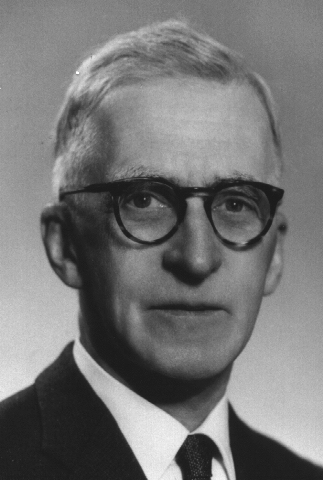
\includegraphics[height=2in]{pitman.jpg}
        % Source: http://www.asap.unimelb.edu.au/bsparcs/aasmemoirs/gifs/pitman.jpg
        %         http://www.asap.unimelb.edu.au/bsparcs/aasmemoirs/pitman.htm
        % License: ???
        % Date accessed: 1/19/2014
        \caption*{E.\ J.\ G.\ Pitman}
    \end{subfigure}%
    ~ 
    \begin{subfigure}[t]{0.33\textwidth}
        \centering
        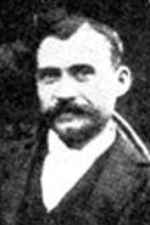
\includegraphics[height=2in]{koopman.jpg}
        % Source: http://cdn4.static.ovimg.com/m/03cnd5k/?width=150
        %         http://www.quazoo.com/q/Bernard_Koopman
        % License: ???
        % Date accessed: 1/19/2014        
        \caption*{Bernard Koopman}
    \end{subfigure}%
    ~
    \begin{subfigure}[t]{0.33\textwidth}
        \centering
        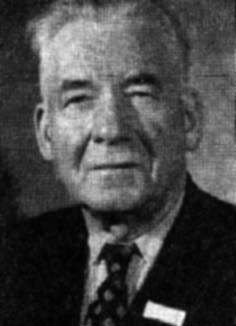
\includegraphics[height=2in]{darmois.jpg}
        % Source: http://www-history.mcs.st-andrews.ac.uk/BigPictures/Darmois_2.jpeg
        %         http://www-history.mcs.st-andrews.ac.uk/Biographies/Darmois.html
        % License: ??? 
        % Date accessed: 1/19/2014
        \caption*{Georges Darmois}
    \end{subfigure}
    % \caption{Caption place holder}
\end{figure}


\section{One-parameter exponential families}

A \term{one-parameter exponential family} is a collection of probability distributions indexed by a parameter $\theta\in\Theta$, such that the p.d.f.s/p.m.f.s are of the form
\begin{align}\label{equation:1d-exponential-family}
p(x|\theta) =\exp\big(\varphi(\theta)t(x)-\kappa(\theta)\big) h(x)
\end{align}
for some functions $\varphi(\theta),t(x),\kappa(\theta)$, and $h(x)$. Note that $\kappa(\theta)$ acts a log-normalization constant---for example, in the continuous case, in order to have $\int p(x|\theta)d x = 1$, it must be that
% todo: derive this? Jurijs didn't find it obvious.
$$\kappa(\theta) = \log \int \exp\big(\varphi(\theta)t(x)\big) h(x)\,d x.$$
Terminology: $t(x)$ is called the \term{sufficient statistic function}.

% \subsubsection*{Example 1: Exponential}
\begin{example}[Exponential]
The $\Exp(\theta)$ distributions form an exponential family, since the p.d.f.s are
$$p(x|\theta) =\Exp(x|\theta) = \theta e^{-\theta x}\I(x>0) =\exp(-\theta x + \log\theta)\I(x>0)$$
for $\theta\in\Theta=(0,\infty)$, and we can put this in the form of Equation \ref{equation:1d-exponential-family} by choosing
\begin{align*}
t(x) &= -x \\
\varphi(\theta) & =\theta \\
\kappa(\theta) & = -\log\theta \\
h(x) &= \I(x>0).
\end{align*}
\end{example}

% \subsubsection*{Example 2: Poisson}
\begin{example}[Poisson]
The $\Poisson(\theta)$ distributions form an exponential family, since the p.m.f.s are
$$p(x|\theta) = \Poisson(x|\theta)= \exp(-\theta)\frac{\theta^x}{x!}\I(x\in S) 
= \exp(x\log\theta - \theta)\I(x\in S)/x!$$
for $\theta\in\Theta=(0,\infty)$, where $S=\{0,1,2,\ldots\}$, and we can choose
\begin{align*}
t(x) &= x \\
\varphi(\theta) & = \log\theta \\
\kappa(\theta) & = \theta \\
h(x) & = \I(x\in S)/x!.
\end{align*}
\end{example}

\subsection{Natural form}
% todo: Do we really need to introduce natural form?

An exponential family is in \term{natural form} (a.k.a. \term{canonical form}) if $\varphi(\theta) =\theta$. In this case, $\theta$ is called the \term{natural parameter}.

% \subsubsection*{Example 1, revisited}
\begin{example}[Exponential]
Choosing $t(x) =-x$ and $\varphi(\theta) = \theta$ as above puts the family $\Exp(\theta)$ in natural form. If we had instead chosen $t(x) = x$ and $\varphi(\theta) = -\theta$, this would not be in natural form.
\end{example}

% \subsubsection*{Example 2, revisited}
\begin{example}[Poisson]
When written as above, the $\Poisson(\theta)$ family is not in natural form. To put it in natural form, we can reparametrize by letting $\eta = \log\theta$. Then 
$$ p(x|\eta) = \exp(x\eta -e^\eta)\I(x\in S)/x!,$$
for $\eta\in\R$, gives us the same collection of probability distributions, and is in natural form, with natural parameter $\eta$.
\end{example}



\section{Conjugate priors}

% todo: clean up this definition---make it clear that it is conjugate FOR a particular generating family.  Make different uses of terminology clear ("conjugate prior", "conjugate to", etc.)
Given a family $\{p(x|\theta):\theta\in\Theta\}$ of generating distributions, a collection of priors $p_\alpha(\theta)$ indexed by $\alpha\in H$ is called a \term{conjugate prior family} if for any $\alpha$ and any data, the resulting posterior equals $p_{\alpha'}(\theta)$  for some $\alpha'\in H$.

% \subsubsection*{Example 1}
\begin{example}[Beta-Bernoulli]
The collection of $\Beta(\theta|a,b)$ distributions, with $a,b>0$, is conjugate to $\Bernoulli(\theta)$, since the posterior is $p(\theta|x_{1:n}) = \Beta(\theta\mid a +\sum x_i, \, b + n-\sum x_i)$.
\end{example}

% \subsubsection*{Example 2}
\begin{example}[Gamma-Exponential]
The collection of $\Ga(\theta|a,b)$ distributions, with $a,b>0$, is conjugate to $\Exp(\theta)$, since the posterior is $p(\theta|x_{1:n}) = \Ga(\theta\mid a+n,\,b+\sum x_i)$.
\end{example}

\subsection{Existence and uniqueness?}
Technically, for any generating family, a conjugate family always exists---namely, the family of all distributions on $\theta$. However, usually when people discuss conjugate priors they mean conjugate families which are computationally-tractable or have a closed-form.
%Simple conjugate priors do not always exist---that is, not every generating family has a conjugate family for which the posterior can be expressed in closed form.

It is also important to recognize that conjugate priors are usually not unique, so it doesn't make sense to talk about ``the conjugate prior'' for a given generating family---instead it is more accurate to discuss ``a conjugate prior''. For instance, suppose $\{p_\alpha(\theta):\alpha\in H\}$ is a conjugate family, and $g(\theta)$ is any nonnegative function. If $0<z(\alpha)<\infty$ for all $\alpha\in H$, where $z(\alpha) = \int p_\alpha(\theta)g(\theta)d\theta$, then
$$\big\{p_\alpha(\theta)g(\theta)/z(\alpha) : \alpha\in H\big\}$$
is also a conjugate family.
A useful special case is to take $g(\theta) =\I(\theta\in A)$ for some set $A$.


\subsection{Conjugate priors for exponential families}
\label{section:conjugate-priors}
\begin{itemize}
\item Under general conditions, any exponential family has a conjugate prior, with p.d.f.
$$p_{n_0,t_0}(\theta) \propto \exp\big(n_0 t_0 \varphi(\theta) - n_0 \kappa(\theta)\big)\I(\theta\in\Theta) $$
% todo: Is this right? (the domain of n_0 and t_0 values)
for the values of $n_0 > 0$ and $t_0\in\R$ for which this is normalizable.
\item However, the normalization constant is not always computationally tractable. Often, when people speak of conjugate priors, it is implied that they mean computationally tractable ones.
\item The resulting posterior is $p_{n',t'}(\theta)$ where $n'=n_0+n$ and 
$$t' = \frac{n_0 t_0 + \sum_{i = 1}^n t(x_i)}{n_0+ n}
 = \frac{n_0}{n_0+ n} t_0 + \frac{n}{n_0+ n}\,\frac{1}{n}\sum_{i = 1}^n t(x_i). $$
Note that this is a convex combination of $t_0$ and $\frac{1}{n}\sum t(x_i)$.
\item This gives us an insight into the interpretation of the prior parameters $t_0$ and $n_0$ that suggests how one might choose them: $t_0$ represents a prior ``guess'' at the expected value of $t(x)$, and $n_0$ represents the prior ``number of samples'' (roughly speaking, how certain we are about $t_0$).
\end{itemize}


\section{Multi-parameter exponential families}

The generalization to more than one parameter is straightforward. An \term{exponential family} is a collection of distributions indexed by $\theta\in\Theta$, with p.d.f.s/p.m.f.s of the form
\begin{align}\label{equation:exponential-family}
p(x|\theta) =\exp\big(\varphi(\theta)^\T t(x)-\kappa(\theta)\big) h(x)
\end{align}
for some vector-valued functions 
\begin{align*}
\varphi(\theta)=\begin{pmatrix}\varphi_1(\theta) \\ \vdots \\ \varphi_k(\theta)\end{pmatrix}
\quad\mbox{ and }\quad
t(x)=\begin{pmatrix}t_1(x) \\ \vdots \\ t_k(x)\end{pmatrix}
\end{align*}
and some real-valued functions $\kappa(\theta)$ and $h(x)$. Here, $v^\T$ denotes the transpose of $v$.
As before, $\kappa(\theta)$ is the log-normalization constant, and the content above regarding natural form and conjugate priors applies also to the multi-parameter case.

% \subsubsection*{Example 1: Beta}
\begin{example}[Beta]
The $\Beta(a,b)$ distributions, with $a,b>0$, are an exponential family:
\begin{align*}
\Beta(x|a,b) &= \frac{1}{B(a,b)}x^{a-1}(1-x)^{b-1}\I(0< x < 1)\\
& = \exp\Big((a-1)\log x + (b-1)\log(1-x)-\log B(a,b)\Big)\I(0< x < 1)
\end{align*}
which can be put in the form of Equation \ref{equation:exponential-family} by choosing, for example, $\theta=(a-1,b-1)^\T$, $\varphi(\theta) = \theta$, $t(x) = (\log x,\log(1-x))^\T$, and $h(x)= \I(0< x < 1)$.
\end{example}

% \subsubsection*{Example 2: Gamma}
\begin{example}[Gamma]
The $\Ga(a,b)$ distributions, with $a,b>0$, are an exponential family:
\begin{align*}
\Ga(x|a,b) & =\frac{b^a}{\Gamma(a)} x^{a-1}\exp(-b x)\I(x>0)\\
& =\exp\Big(-b x +(a-1)\log x +\log\frac{b^a}{\Gamma(a)}\Big)\I(x>0),
\end{align*}
and we can choose, for example, $\theta=(a,b)^\T$, $\varphi(\theta) = (-b,a-1)^\T$, $t(x) = (x,\log x)^\T$, and $h(x)= \I(x>0)$.
\end{example}



%\section{Motivations for using exponential families}
%\todo{finish}




\section{Exercises}

\begin{enumerate}
\item Show that the $\Bernoulli(\theta)$ distributions form a \textit{one-parameter} exponential family.
\item If $X_1,\dotsc,X_n\iid\Bernoulli(\theta)$, then the distribution of the sum $Z =\sum_{i = 1}^n X_i$ has the $\Binomial(n,\theta)$ distribution. Show that with $n$ fixed, the $\Binomial(n,\theta)$ distributions form a one-parameter exponential family.
\item Consider the $\Ga(a,b)$ distributions with $a$ fixed. Find a conjugate prior for $b$.
\item Show that for a certain choice of $t(x)$ and $h(x)$, the $\Ga(a,b)$ distributions are in natural form with natural parameter $\theta =(a,b)^\T$.
\item Section \ref{section:conjugate-priors} presented the general form of the posterior for a one-parameter exponential family with a conjugate prior. Derive this.
\item Suppose $\{p_\alpha(\theta):\alpha\in H\}$ is a conjugate family for some generator family $\{p(x|\theta):\theta\in\Theta\}$, let $g(\theta)$ be a nonnegative function, and define $z(\alpha) =\int p_\alpha(\theta) g(\theta) d\theta$.  Show that if $0<z(\alpha)<\infty$ for all $\alpha\in H$, then
$$\big\{p_\alpha(\theta)g(\theta)/z(\alpha) : \alpha\in H\big\}$$
is also a conjugate family.
\item Suppose $\{p_\alpha(\theta):\alpha\in H\}$ is a conjugate family for some generator family. Show that the following is also a conjugate family for the same generator family:
$$\Big\{\sum_{i = 1}^k \pi_i p_{\alpha_i}(\theta) \,:\, \alpha_1,\dotsc,\alpha_k\in H, \, \pi\in\Delta_k\Big\} $$
where
$$\Delta_k =\Big\{\pi\in\R^k\,:\,\pi,\dotsc,\pi_k\geq 0, \, \sum_{i = 1}^k \pi_i = 1\Big\}. $$
In other words, finite mixtures of conjugate priors are conjugate priors. This enables one to construct very flexible classes of conjugate priors.
\end{enumerate}








\section*{Supplementary material}

% \subsubsection*{}
\begin{itemize}
\item Hoff (2009), Section 3.3.
%\item \url{http://en.wikipedia.org/wiki/Exponential_family}
%\item \url{http://en.wikipedia.org/wiki/Conjugate_prior}
\end{itemize}

\section*{References}

\begin{itemize}
\item Diaconis, P., \& Ylvisaker, D. (1979). Conjugate priors for exponential families. The Annals of Statistics, 7(2), 269-281.
\item Orbanz, P., (2009), Functional Conjugacy in Parametric Bayesian Models.
\item Hoffman-Jorgensen, J. (1994). Probability with a view towards statistics. CRC Press.
\end{itemize}

\subsubsection*{Historical publications}
\begin{itemize}
\item Pitman, E. J. G. (1936). Sufficient statistics and intrinsic accuracy. In Mathematical Proceedings of the Cambridge Philosophical Society (Vol. 32, No. 04, pp. 567-579). Cambridge University Press.
\item Koopman, B. O. (1936). On distributions admitting a sufficient statistic. Transactions of the American Mathematical Society, 39(3), 399-409.
\item Darmois, G. (1935). Sur les lois de probabilite a estimation exhaustive. CR Acad. Sci. Paris, 260, 1265-1266.
\end{itemize}



\end{document}






